% This is samplepaper.tex, a sample chapter demonstrating the
% LLNCS macro package for Springer Computer Science proceedings;
% Version 2.21 of 2022/01/12
%
\documentclass[runningheads]{llncs}
%
\usepackage[T1]{fontenc}
\usepackage{verbatim}  % Required for the verbatim environment
% T1 fonts will be used to generate the final print and online PDFs,
% so please use T1 fonts in your manuscript whenever possible.
% Other font encodings may result in incorrect characters.
%
\usepackage{graphicx}
\usepackage{natbib}
\usepackage{amsmath}
% Used for displaying a sample figure. If possible, figure files should
% be included in EPS format.
%
% If you use the hyperref package, please uncomment the following two lines
% to display URLs in blue roman font according to Springer's eBook style:
%\usepackage{color}
%\renewcommand\UrlFont{\color{blue}\rmfamily}
%\urlstyle{rm}
%
\begin{document}
%
\title{Studiul Algoritmilor de Rezolvare SAT și Implementarea lor în MiniSat}
%
%\titlerunning{Abbreviated paper title}
% If the paper title is too long for the running head, you can set
% an abbreviated paper title here
%
%Haiosta Michelle, Cerean Bogdan-Ioan, Popovici Adrian-Robert, Bosna Marinel
\author{Haiosta Michelle \and
Cerean Bogdan-Ioan \and
Popovici Adrian-Robert \and
Bosna Marinel}


\institute{West University of Timișoara}
%
\maketitle              % typeset the header of the contribution
%

\section*{Abstract}
\paragraph{Lucrarea} prezintă o introducere scurtă în probleme de tip SAT și analizează SAT Solverul MiniSat, prezentând modul de instalare a programului, o analiză asupra codului și posibile modalități de a îmbunătății acest program.

\keywords{MiniSat  \and SAT Solver \and Logică propozițională.}

\newpage
%
%
%

\section{Introducere}
\paragraph{În această lucrare este prezentat SAT Solverul MiniSat}, un program folosit pentru a rezolva probleme de verificare formală cât și în competiții de rezolvare a problemelor SAT. Lucrarea este împărțită în 6 secțiuni care adresează aspectele acestei aplicații: 

\begin{enumerate}
    \item Primul capitol este o prezentare a MiniSat-ului  și o introducere a problemelor de tip SAT.
    \item Al doilea capitol este o explicație a procesului de instalare și pregătire a MiniSat pentru a-l putea folosi în practică.
    \item Al treilea capitol descrie modul de folosire a aplicației pentru a rula un benchmark, un set de probleme folosite în competiții SAT pentru a testa eficiența unui SAT Solver.
    \item Al patrulea capitol conferă o analiză asupra codului și logici programului MiniSat, incluzând o diagramă care arată pas cu pas ordinea apelării funcțiilor în program și o descriere a fiecărei metode în parte.
    \item Al cincilea capitol discută posibile metode de a îmbunătății SAT Solver-ul, tema competițiilor anuale de SAT unde mai multe echipe prezintă algoritmi modificați sau programe originale de rezolvare a problemelor de tip SAT.
    \item Ultimul capitol, capitolul 6, este o încheiere în care sunt discutate dificultăți întâlnite în timpul compunerii acestei lucrări.
\end{enumerate}


\section{Descrierea problemei}
\paragraph{Problemele de satisfiabilitate}, cunoscute și ca probleme SAT, sunt probleme în care analizăm o propoziție logică, formată din una sau mai multe clauze aflate în conjuncție. Fiecare clauză conține literali aflați în disjuncție. Un literal reprezintă fie o variabilă, fie o negare de variabilă. Acest format, în care avem doar conjuncții, disjuncții și negări este cunoscut ca Forma Normală Conjunctivă sau CNF. \cite{biere2009handbook}

\paragraph{În urma analizei}, care implică acordarea de valori True sau False variabilelor propoziției în diferite combinații, ne așteptăm să găsim o combinație de variabile care satisface fiecare clauză a propoziției. Dacă fiecare clauză este satisfăcută, propoziția finală este adevărată, ceea ce înseamnă că această problemă este satisfiabilă, sau SAT. Dacă nu există o combinație de variabile în care propoziția să fie adevărată, adică dacă nu avem o soluție a problemei, ea este considerată nesatisfiabilă sau UNSAT. \cite{zhang2013boolean}

\paragraph{Problemele de tip SAT} sunt folosite în domenii cum ar fi inteligența artificială, proiectarea de circuite și Automated Theory Proving (ATP). În aceste domenii pot apărea probleme care au zeci de mii de variabile și sute de mii de simboluri. În rezolvarea manuală apar dificultăți chiar și când o problemă are doar zece variabile, iar complexitatea și timpul necesar pentru a rezolva o problemă SAT ar fi enorme, chiar și când aplicăm algoritmi cum ar fi CDCL sau DPLL. Din acest motiv, programe de tip SAT Solver, care pot analiza probleme SAT în mod automat și rapid, au fost dezvoltate și încă sunt folosite în prezent. Domeniul problemelor SAT este foarte studiat, existând concursuri anuale în care SAT Solvere sunt puse în competiție pentru a vedea care rulează mai eficient pe seturi de date enorme numite benchmark-uri.

\paragraph{MiniSat} este un astfel de SAT Solver, gratuit și open-source, dezvoltat de Niklas Een și Nikita Sorensson în 2003 și publicat în 2004, folosit atât academic, cât și în industrie. Acest program a fost dezvoltat ca fiind un SAT Solver extensibil, care să poată fi modificat și adaptat la diverse domenii mult mai rapid, comparabil cu alte Solvere contemporane sau alternativa de a crea un Solver nou de la zero. MiniSat rulează în Linux, iar instalarea sa este prezentată în capitolul următor. \cite{eensorensson2005minisat} \cite{eensorensson2003extensible}

\section{Instalarea MiniSat}

\paragraph{Pentru a rula MiniSat,} este necesar să folosim o distribuție Linux. Putem folosi o mașinărie virtuală pentru a rula MiniSat, dar o metodă mult mai simplă este „Windows Subsystem for Linux”, abreviat WSL, care ne permite să rulăm un environment Linux fără a folosi o mașinărie virtuală sau paralel booting. \cite{minisatmanual}

\paragraph{Instalarea WSL} se poate executa direct din PowerShell sau Windows Command Prompt, folosind comanda „WSL --install” care, după repornirea sistemului, va instala pe calculator o distribuție Ubuntu. Dacă dorim să folosim altă distribuție, este suficient să folosim comanda: \texttt{WSL --install <Numele distribuției>}

%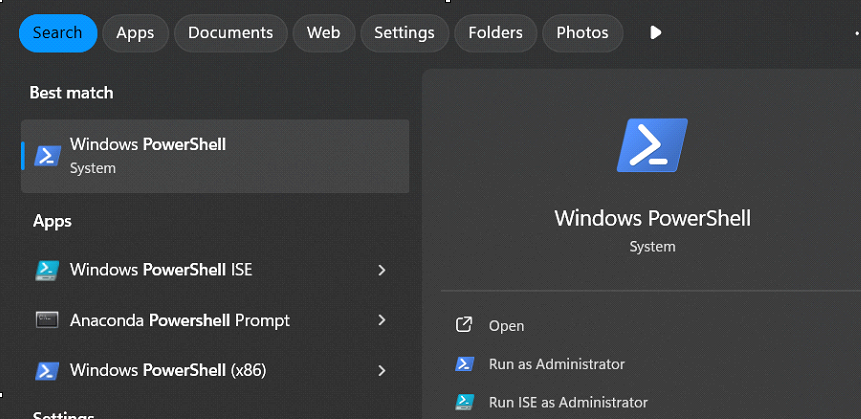
\includegraphics[width=\textwidth]{images/3_instalare/1.png}
\begin{figure}
    \centering
    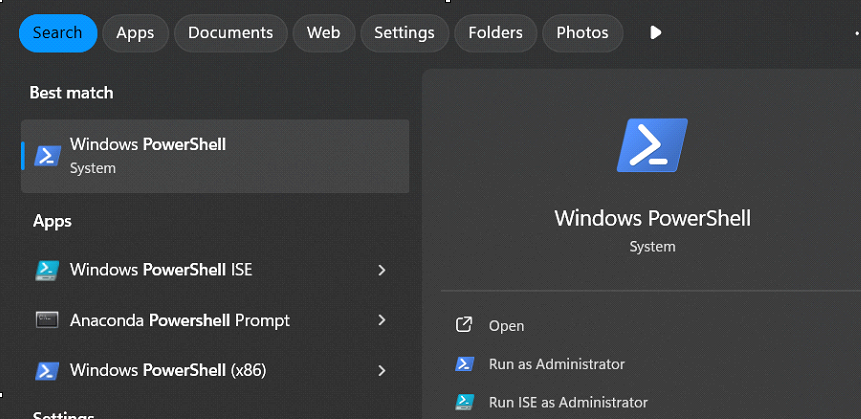
\includegraphics[width=0.75\linewidth]{images/3_instalare/1.png}
    \caption{Fereastra selectare WindowsPowerShell}
    \label{fig:2}
\end{figure}

\begin{figure}
    \centering
    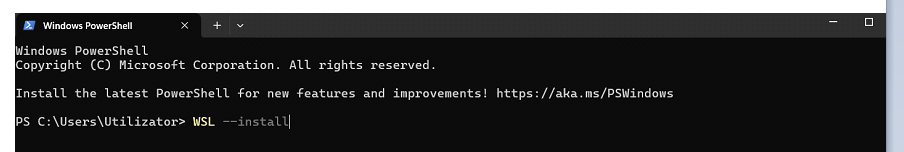
\includegraphics[width=0.75\linewidth]{images/3_instalare/2.png}
    \caption{Instalare WSL}
    \label{fig:enter-label}
\end{figure}

Odată ce am instalat WSL și am repornit calculatorul, putem folosi aplicația WSL pentru a accesa distribuția Ubuntu pe care o avem. Odată ce accesăm linia de comandă, fie folosind WSL, fie o mașină virtuală, MiniSat poate fi instalat folosind managerul de pachete Linux. Putem actualiza managerul de pachete folosind comanda \texttt{sudo apt update}, după care instalarea MiniSat necesită o singură comandă: \texttt{sudo apt install minisat}

\begin{center}
    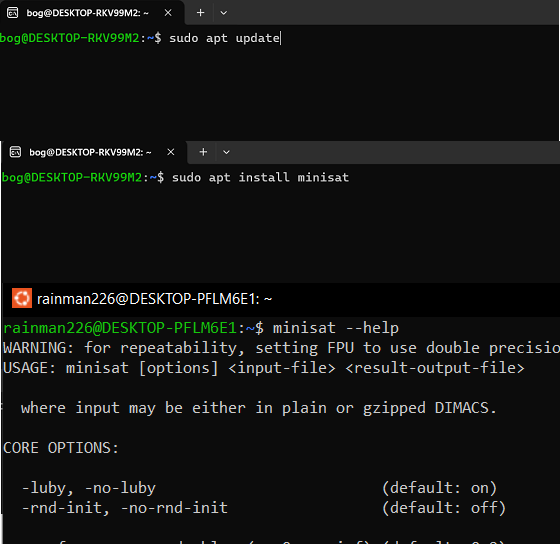
\includegraphics[width=0.75\textwidth]{images/3_instalare/3.png}
\end{center}

\section{Rularea benchmark}
 
MiniSat este un SAT solver simplu, dar foarte eficient. Pentru a înțelege mai bine cum funcționează și cât de bine face față problemelor complexe, am rulat un benchmark din competiția SAT pentru a analiza performanța și comportamentul său. 
 
Competiția SAT \cite {satcompetition} este un concurs internațional în care cei mai buni solvers SAT sunt evaluați pe un set de benchmark-uri standardizate, pentru a testa eficiența și corectitudinea algoritmilor. Aceste benchmark-uri sunt gândite pentru a acoperi o varietate de probleme complexe și pentru a stimula dezvoltarea unor soluții mai rapide și mai eficiente.

 \subsection{Descriere benchmark folosit}
În cadrul acestui test, am folosit un benchmark bazat pe "Simon Cipher" — o schemă criptografică de tip block cipher, care utilizează o structură echilibrată de tip Feistel și operații pe blocuri de biți prin porți logice AND și XOR. Acest tip de schemă este cunoscut pentru simplitatea implementării sale și eficiența sa pe dispozitive de tip Internet of Things, menținând un nivel de securitate acceptabil.

Pentru a adapta problema la formatul SAT și a genera instanțe cu dificultate moderată, s-a simplificat schema originală a algoritmului. Această simplificare a implicat reducerea numărului de runde, eliminarea procesului de programare a cheilor (key scheduling) și utilizarea unui set de stări inițiale prestabilite. Cheia utilizată pentru toate rundele a fost compusă exclusiv din biți de valoare 1 (all-1 key), iar numărul de runde a fost redus la un interval de 16 până la 25. Aceste ajustări asigură că instanțele pot fi rezolvate de către majoritatea solverelor SAT moderne într-un timp rezonabil, păstrând totodată caracteristicile esențiale ale problemei.

\begin{figure}
    \centering
    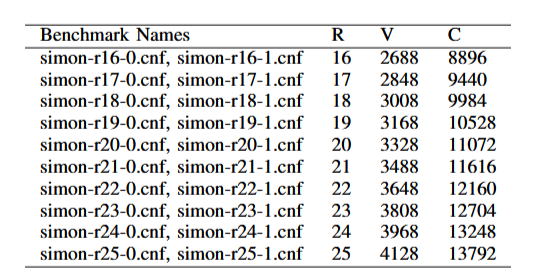
\includegraphics[width=0.5\linewidth]{images/benchmark/tabel date.png}
    \caption{Detalii instanțe}
    \label{fig:enter-label}
\end{figure}

Benchmarks-urile prezentate sunt afișate în Fig. 3, unde sunt indicate numărul de runde (R), numărul de variabile (V) și numărul de clauze (C). Pentru fiecare rundă, creăm aleatoriu două instanțe folosind două semințe diferite.
Aceste instanțe au fost concepute pentru a evidenția performanțele solverelor SAT în fața problemelor criptografice cu o structură bine definită, dar suficient de simplificate pentru a fi analizate eficient.

\subsection{Metodologia de rulare extinsă}

Pentru a evalua performanța MiniSat pe benchmark-urile selectate, am efectuat experimentele într-un interval total de 24 de ore. Am avut la dispoziție 10 fișiere de benchmark, fiecare fiind rulat cu o limită de timp de 8.460 secunde folosind comanda:
\begin{verbatim}
minisat -cpu-lim=8640 "$benchmark" "$output".
\end{verbatim}
Testele au fost efectuate pe un calculator echipat cu procesor AMD Ryzen 5 4600H și 8 GB RAM, resurse suficiente pentru monitorizarea eficientă a performanței MiniSat.

Pentru a optimiza rulările și a obține rezultate mai eficiente, am utilizat câțiva parametri recomandați dintr-un articol de cercetare \cite{beskydsurynek2023parameter} care analizează impactul setărilor asupra performanței solverului. Acești parametri ajustează euristici cheie ale MiniSat, având o influență semnificativă asupra timpului de rulare. Iată explicațiile acestora:
\begin{itemize}
    \item \texttt{-var-decay} (factorul de decădere al variabilelor):\\
    Acest parametru controlează frecvența cu care activitatea variabilelor scade după conflicte. Activitatea variabilelor reflectă frecvența cu care acestea apar în conflicte recente. Un factor de decădere mai mic face ca variabilele recente să rămână relevante pentru mai mult timp.\\
    \textbf{Valoare optimă recomandată:} \texttt{-var-decay=0.95}.
    
    \item \texttt{-cla-decay} (factorul de decădere al clauzelor):\\
    Similar cu variabilele, activitatea clauzelor crește atunci când acestea sunt implicate în conflicte și scade periodic în funcție de acest factor de decădere. Un factor de decădere bine ajustat ajută la eliminarea clauzelor inactive, optimizând astfel performanța solverului.\\
    \textbf{Valoare optimă recomandată:} \texttt{-cla-decay=0.93}.
    
    \item \texttt{-rfirst} (intervalul de restart inițial):\\
    Determină numărul de conflicte care trebuie să apară înainte de prima reluare a căutării (restart). Restart-urile frecvente pot ajuta solverul să evite blocarea într-o regiune a spațiului de căutare dificilă de rezolvat.\\
    \textbf{Valoare optimă recomandată:} \texttt{-rfirst=200}.
\end{itemize}

Pe baza acestor recomandări, am configurat rulările benchmark-urilor folosind comanda:
\begin{verbatim}
minisat -var-decay=0.95 -cla-decay=0.93 -rfirst=200 "$benchmark" "$output".
\end{verbatim}

Aceste setări au fost alese deoarece optimizările propuse permit MiniSat să exploateze mai bine structura instanțelor, îmbunătățind atât numărul de conflicte rezolvate, cât și timpul total de rulare.

\subsection{Interpretarea valorilor rezultate din rulare}
 
Pentru a evalua performanța MiniSat pe setul de benchmark-uri, am analizat log-urile generate de solver, concentrându-ne pe unele statistici. Datele colectate pot fi împărțite în două părți: statisticile problemei și statisticile rezolvării. Statisticile problemei oferă informații despre configurația inițială a fiecărei instanțe SAT, în timp ce statisticile rezolvării urmăresc progresul solverului în timpul procesului de rezolvare.
 
Următorii parametri reprezintă caracteristicile de bază ale instanței SAT analizate:
 
\begin{itemize}
    \item \textbf{Variables}: numărul total de variabile din formula SAT, care indică complexitatea problemei și dimensiunea spațiului de căutare a soluției.
    \item \textbf{Clauses}: Reprezintă numărul total de clauze din formula SAT, ceea ce determină câte relații logice există între variabile. Cu cât sunt mai multe clauze, cu atât problema devine mai complexă și dificilă.
\end{itemize}
 
Iar statisticile relevante rezolvării:
 
\begin{itemize}
    \item \textbf{Restarts}: Restarturile sunt strategii de reînnoire a procesului de căutare pentru a evita blocajele în soluționare și pentru a explora mai eficient spațiul soluțiilor.
    \item \textbf{Conflicts}: Numărul total de conflicte întâmpinate. Conflictele apar atunci când solverul identifică o contradicție în setul curent de alocări, ceea ce forțează revenirea (backtracking) și ajustarea traseului de căutare.
    \item \textbf{Decisions}: Numărul total de decizii făcute. Reprezintă alegerile pe care solverul le face pentru a atribui valori variabilelor. Numărul ridicat de decizii reflectă o căutare extinsă a soluției.
    \item \textbf{Propagations}: Numărul de propagări efectuate. Pași intermediari prin care o decizie influențează alte variabile, reducând spațiul posibil al soluțiilor și avansând soluționarea.
    \item \textbf{Conflict literals}: Numărul total de literali conflictuali. Sunt literali care au condus la conflicte și care pot fi eliminați pentru a simplifica problema.
    \item \textbf{Memory used}: Memoria utilizată de solver în timpul execuției.
    \item \textbf{CPU time}: Timpul total de procesare alocat execuției.
    \item \textbf{Result}: Rezultatul final al solverului.
\end{itemize}

 \subsection{Rezultate rulare benchmark}

 
\begin{center}
    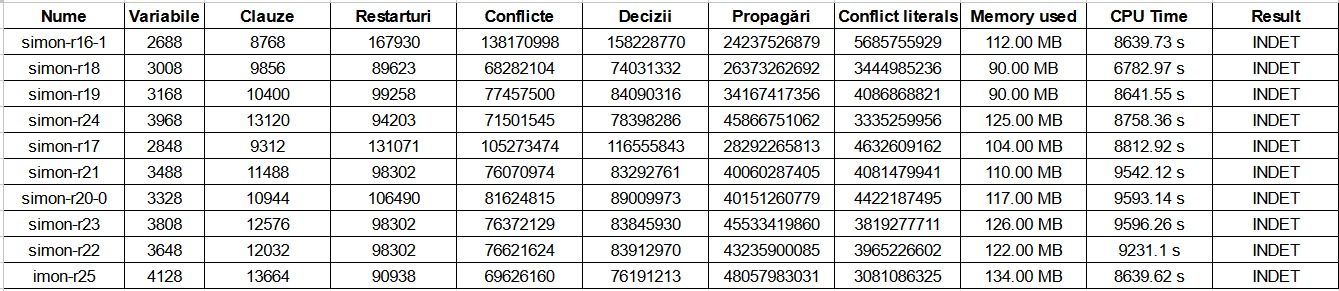
\includegraphics[width=1.20\textwidth]{images/benchmark/tabel_rezultate.jpg}
     \caption{Tabel cu rezultate}
\end{center}
 
Rezultatele obținute arată că MiniSat a reușit să proceseze benchmark-urile complexe în limitele de timp și memorie specificate, dar pentru toate instanțele testate soluția nu a fost determinată în intervalul de timp alocat, fiind returnat rezultatul INDETERMINATE. Acest lucru evidențiază dificultatea extremă a problemelor abordate, fiecare necesitând un număr foarte mare de conflicte, decizii și propagări pentru a explora spațiul soluțiilor.

Se observă o corelație clară între dimensiunea instanțelor și dificultatea lor. De exemplu, instanțele cu mai multe variabile și clauze, cum ar fi simon-r25 cu 4128 variabile și 13664 clauze, au necesitat un volum mult mai mare de propagări și conflicte în comparație cu instanțe mai mici, precum simon-r16-1 cu 2688 variabile și 8768 clauze. Această creștere a dificultății este confirmată de numărul ridicat de conflicte și decizii pentru instanțele mari, cum sunt simon-r24 (71501545 conflicte și 78398268 decizii) sau simon-r25 (69626160 conflicte și 76191213 decizii). De asemenea, numărul mare de restarturi, cum ar fi 167930 pentru simon-r16-1 și 131071 pentru simon-r17, reflectă provocările întâlnite de solver în evitarea blocării în regiuni dificile ale spațiului de căutare.

În ceea ce privește utilizarea resurselor, memoria folosită a fost relativ scăzută, variind între 90 MB și 134 MB, ceea ce indică o bună eficiență în gestionarea resurselor hardware. Totuși, timpul de procesare s-a apropiat de limita alocată pentru fiecare instanță, de exemplu 8639,73 secunde pentru simon-r25, sugerând că algoritmul folosit de MiniSat nu este suficient de rapid pentru a rezolva astfel de probleme complexe într-un interval de timp rezonabil.

Aceste rezultate subliniază necesitatea unor optimizări suplimentare ale euristicilor folosite de MiniSat sau chiar a utilizării unor metode mai avansate. Spre exemplu, integrarea unor algoritmi mai sofisticați sau utilizarea unor tehnici bazate pe învățare automată ar putea contribui la reducerea spațiului de căutare și la îmbunătățirea performanței.

\section{Analiza Cod}

În imaginea de mai jos este prezentată o schiță a algoritmului de search din codul MiniSat \cite{minisatgithub} , prezentată sub forma de pseudo-cod. Imaginea ne va ajuta să înțelegem pașii principali pe care acest algoritm îi urmează pentru a încerca, verifica și învăța din greșeli până când se găsește o soluție sau până când se demonstrează că nu există nicio soluție.

\begin{center} 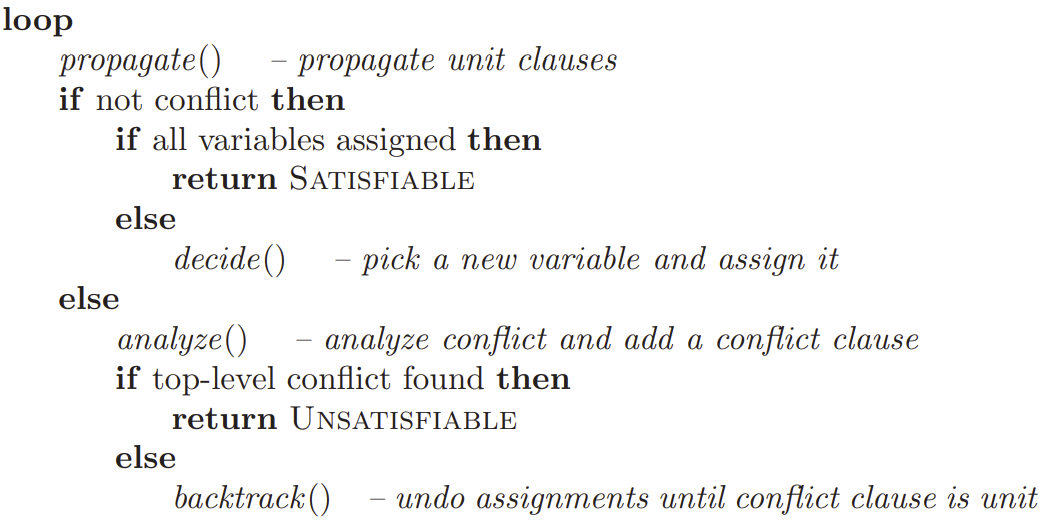
\includegraphics[width=0.75\textwidth]{images/diagrams/pseudo_code/search_pseudo.png} \end{center}

Pentru a înțelege mai în detaliu fluxul acestui algoritm am creat diagrama de secvențe de mai jos, unde avem actorul principal (Solverul) și restul componentelor participante la algoritmul de search: Baza de date a clauzelor, Analizatorul de conflicte, Coada de literali și Managerul de nivel decizional:

\begin{center} 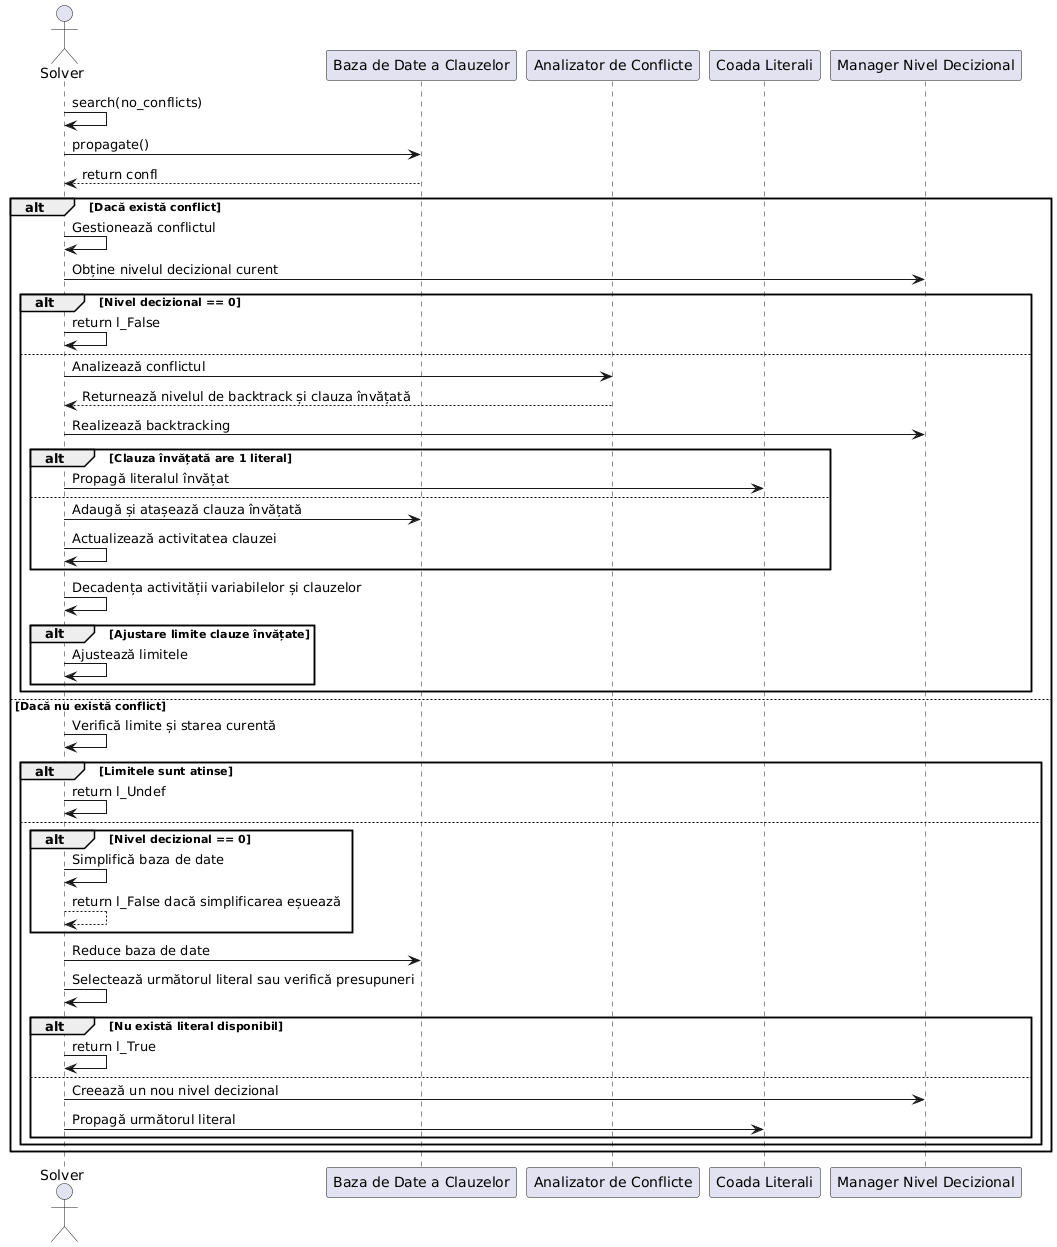
\includegraphics[width=1.0\textwidth]{images/diagrams/search_romana_2.png} \caption{Diagrama de secvențe pentru metoda search} \end{center}

Am observat, uitându-ne la codul proiectului MiniSat, că acesta se folosește de algoritmul CDCL, iar în fișierul solver.cc din directorul core, acest algoritm este bine evidențiat prin metoda search. Pentru a înțelege mai bine cum funcționează \textbf{search()}, vom descrie fiecare etapă importantă din acest proces. \cite{eensorensson2005minisatreport}

Această metodă explorează diferite combinații de valori pentru variabilele din formulă pentru a determina dacă există o soluție care să satisfacă toate clauzele sau, în caz contrar, că formula este nesatisfiabilă. Algoritmul urmează mai mulți pași, iar fiecare componentă joacă un rol esențial în procesul de căutare.

\subsection{Inițializare} La început, \textbf{search()} inițializează mai multe variabile de lucru, precum \textbf{conflicts}, care este contorul de conflicte, și \textbf{learnt\_clause}, folosită pentru stocarea clauzei conflictuale curente în timpul analizei.

\textbf{Cazul special} este dacă nu există clauze de la început, algoritmul concluzionează că formula este satisfiabilă deoarece o formulă fără clauze este implicit satisfăcută. În acest caz, metoda \textbf{search()} returnează o soluție imediat, evitând astfel execuția restului algoritmului.

\subsection{Propagare (funcția propagate())} Propagarea este următorul pas în proces, aplicată pentru a deduce valori pentru variabile pe baza clauzelor existente. \textbf{propagate()} încearcă să seteze valori noi pentru variabile, verificând în același timp dacă aceste setări satisfac clauzele deja existente. Propagarea unitară este o tehnică esențială folosită în metodă pentru a determina valoarea variabilelor.

\textbf{Cazul special} este dacă \textbf{propagate()} detectează un conflict (adică o clauză are toți literalii falși), metoda returnează o referință la acea clauză conflictuală. În acest caz, \textbf{search()} trece la analiza conflictului pentru a învăța o clauză nouă care să evite conflictele similare în viitor.

\subsection{Gestionarea conflictului} Când \textbf{propagate()} returnează o clauză conflictuală, \textbf{search()} apelează \textbf{analyze()} pentru a determina cauza conflictului. În acest pas, \textbf{analyze()} examinează variabilele implicate și construiește o nouă clauză numită clauză de conflict. Aceasta este adăugată la baza de date de clauze și este destinată să prevină conflictele similare în viitor.

\textbf{Cazul special} este dacă conflictul apare la nivelul de decizie 0, adică la nivelul de bază al algoritmului, \textbf{search()} concluzionează că formula este nesatisfiabilă. În această situație, funcția se oprește și returnează UNSAT, deoarece nu există nicio configurație a variabilelor care să satisfacă formula.

\subsection{Învățarea clauzei de conflict și backtracking-ul (funcția analyze())} Funcția \textbf{analyze()} parcurge clauza conflictuală (\textbf{conflict\_clause}) și variabilele aferente pentru a construi o clauză nouă care să împiedice conflicte similare. În acest mod, solverul CDCL devine mai eficient pe măsură ce își „amintește” conflictele trecute.

\textbf{Cazul special} este după crearea clauzei de conflict, \textbf{search()} stabilește la ce nivel de decizie să revină (backtracking) pentru a evita conflictul. Această revenire la un nivel anterior de decizie permite algoritmului să încerce un alt set de decizii, explorând astfel o altă parte a spațiului soluțiilor.

\subsection{Curățarea bazei de date de clauze (funcția reduceDB())} Pentru a evita acumularea de clauze care încetinesc algoritmul, \textbf{search()} apelează \textbf{reduceDB()} la intervale regulate. Funcția \textbf{reduceDB()} șterge clauzele cu activitate scăzută, adică acelea care nu contribuie semnificativ la prevenirea conflictelor.

\textbf{Cazul special:} Dacă baza de date de clauze devine prea mare, \textbf{reduceDB()} elimină clauzele mai puțin relevante, asigurând o performanță optimă pe termen lung. Acest proces ajută algoritmul să fie mai eficient în gestionarea memoriei și a timpului de execuție.

\subsection{Decizie pentru variabilă (funcția pickBranchLit())} Dacă nu sunt găsite conflicte în propagare și nu au fost setate toate variabilele, \textbf{search()} selectează o variabilă de decizie folosind \textbf{pickBranchLit()}. Această funcție se bazează pe activitatea variabilelor (cele implicate frecvent în conflicte recente), măsurată în funcție de frecvența cu care variabilele au fost implicate în conflicte recente. Variabilele cu activitate ridicată sunt prioritizate pentru a spori eficiența căutării. Setarea acestei variabile contribuie la avansarea în căutare și la explorarea spațiului soluțiilor.

\textbf{Cazul special} Dacă toate variabilele au fost setate fără a apărea conflicte, \textbf{search()} returnează SAT, indicând că formula este satisfiabilă.

\subsection{Restarturi}
  Restarturile se declanșează atunci când numărul de conflicte întâlnite de solver depășește un prag predefinit. Acest prag poate fi stabilit, sau fix, sau ajustat dinamic, în funcție de progresul solverului. Acesta constă în revenirea la nivelul de decizie inițial (0) și începerea unei noi explorări a spațiului soluțiilor. Toate clauzele de conflict învățate sunt păstrate, astfel încât algoritmul să folosească aceste informații în căutarea ulterioară. Restarturile sunt o strategie pentru a evita blocarea într-o regiune specifică a căutării și pentru a explora noi rute de soluții.

\textbf{Cazul special} dacă numărul de conflicte depășește un prag stabilit, algoritmul execută un restart și revine la nivelul de decizie 0, reluând căutarea, dar păstrând clauzele conflictuale învățate.

\subsection{Finalizarea căutării} Dacă \textbf{search()} găsește o setare a variabilelor care satisface toate clauzele, algoritmul returnează \textbf{l\underline{ }True}, indicând că formula este SAT. Pe de altă parte, dacă la nivelul de decizie 0 apare un conflict și nu mai există alte căi de explorat, algoritmul conchide că formula este UNSAT și returnează \textbf{l\underline{ }False}.

\section{Doxygen}
\subsection{Ce este Doxygen?}
Doxygen \cite{doxygenmanual} este un generator de documentație care funcționează pe mai multe limbaje de programare printre care și c++ sau c, limbaje cu care a fost scrisa implementarea MiniSat. Acest generator de documentații extrage comentariile formatate din codul sursă pe care dezvoltatorul software le adauga și salvează toate aceste informații într-un format acceptat, în cazul nostru formatul în care Doxygen salvează informațiile este .html și latex, de asemenea se consideră faptul că Doxygen acceptă analiza statică a unei baze de cod.
\subsection{De ce am ales să documentăm codul cu Doxygen?}
Doxygen este unul dintre cele mai populare instrumente de documentare a codului folosit în dezvoltarea software, însă motivația principală în alegerea folosirii Doxygen a fost dată de faptul că MiniSat nu are nici un fel de documentație a codului în nici un fel de format, de asemenea în formatul generat de Doxygen cu documentația codului se poate include și fișierul read.me ceea ce oferă niște informații clare despre proiect, benchmarkuri și niște pași clari în instalarea MiniSat pe computerul personal.
\subsection{Cum am instalat Doxygen?}
Pentru instalarea Doxygen pe Windows trebuie să accesăm site-ul lor official: https://www.doxygen.nl/download.html și să descărcăm executorul. După rularea executorului trebuie să urmăm pașii pentru instalarea lui pe computerul personal. După finalizarea pașilor de instalare trebuie să adăugam în environment variables path-ul către directoriul Doxygen. Insă pentru instalarea Doxygen pe Linux putem să utilizăm managerul de pachete folosind comanda: sudo apt install doxygen, iar pe macOS putem să instalam Doxygen folosind Homebrew ruland: brew install doxygen.
După instalarea Doxygen trebuie să parcurgem niște pași de configurare:
\begin{enumerate}
    \item Navigare în directorul proiectului nostru.
    \item Generarea fișierului de configurare Doxyfile folosind: doxygen -g. Doxyfile este fișierul de configurare care conține toate setările proiectului nostru.
    \item Generarea setărilor documentației. După ce ne-am configurat fișierul Doxyfile pentru generarea documentației cum ar fi definirea fișierelor pe care dorim să le includem în documentația noastră, tipul documentației pe care dorim să îl generăm (latex, html, xml, etc.), sau putem configura setări customizabile pentru cum vrem să arate documentația noastră (putem genera documentația doar pentru metode sau atribute cu un anumit nivel de vizibilitate). 
    \item Generarea fișierelor de documentație folosind comanda: doxygen Doxyfile. După rularea comenzii se vor genera fișierele html și latex. Pentru vizualizarea documentației în format html trebuie să intram în directorul html și să accesam fișierul index.html, dacă am optat pentru configurarea documentației în latex in fișierul de configurare Doxyfile atunci se va genera și un fisier latex pe care îl putem accesa pentru vizualizarea documentației codului în latex. Fișierul latex se poate converti în format zip și încarca în orice fel de editor (ex: Overleaf).
    \item După fiecare acutalizare a codului pentru actualizarea documentației trebuie să rulam din nou comanda: doxygen Doxyfile în fișierul sursă al codului.
\end{enumerate}

\subsection{Cum am comentat codul folosind Doxygen}
Comenzi utile pentru utlizarea Doxygen:
\begin{itemize}
    \item \textbf{doxygen -g}: aceasta comandă ne creaza fișierul de configurație Doxyfile în directorul unde rulăm comanda. Fișier ce conține toate setările de generare a documentației.
    \item \textbf{doxygen Doxyfile}: această comandă rulează fișierul de configurație conform setărilor din interiorul său și generează documentația în formatul dorit.
    \item \textbf{GENERATE\_LATEX = YES}: această comandă convertește fișierele latex în fișiere pdf care pot fi vizualizate fără un editor precum Overleaf.
    \item \textbf{HAVE\_DOT = YES}: această comandă ne permite generarea automată a diagramelor de clasă folosind Graphviz.
\end{itemize}
Tag-uri utile pentru gestionarea fișierelor de cod:
\begin{itemize}
    \item \textbf{@file}: acest tag se ocupă de descrierea unui fișier sursă. Exemplu: 
    \begin{verbatim}
    /**
     * @file Solver.cc
     * @brief Implementarea MiniSat SAT solver.
     * 
     * Acest fișier conține cele mai importante metode pentru rezolvarea problemelor SAT.
    */
    \end{verbatim}
    \item \textbf{@class}: acest tag descriere rolul și funcționalitatea unei clase.
    Exemplu:
    \begin{verbatim}
     /**
     * @class Solver
     * @brief Clasa principală pentru rezolvarea problemelor SAT.
     * 
     */
    \end{verbatim}
    \item \textbf{@brief, @param, @return}: \textbf{@brief} se ocupă cu descrierea unei funcții sau clase, \textbf{@param} se ocupă cu descrierea parametriilor unei funcții, \textbf{@return} se ocupă cu precizarea tipului de return a unei funcții.
    \begin{verbatim}
    /**
     * @brief Realizează propagarea tuturor literali puși în coadă.
     * 
     * @param level Nivelul decizional curent.
     * @return CRef Referință la clauza conflictuală dacă există un conflict; altfel, CRef_Undef.
     */
    CRef propagate(int level);
    \end{verbatim}
    \item \textbf{@see, @ref}: \textbf{@see} sau \textbf{@ref} creează legături între funcții, clase sau orice alt tip de fișier din cod.
    Exemplu:
    \begin{verbatim}
    /**
    * @brief Algoritmul principal de căutare.
    * 
    * @see propagate()
    * @see analyze()
    */
    lbool search(int nof_conflicts);
    \end{verbatim}
    \item \textbf{@note, @warning}: acest tag se ocupă cu evidențierea lucrurilor mai importante sau cu atenționarea la diferite riscuri.
    Exemplu:
    \begin{verbatim}
    /**
     * @note Această funcție este optimizată pentru probleme mici.
     * @warning Utilizarea pentru probleme mari poate duce la performanțe scăzute.
     */
    void optimizeDatabase();
    \end{verbatim}
\end{itemize}
\section{Procesul de Compilare, Rulare și Interpretare a Rezultatelor MiniSat}

Am configurat și rulat în detaliu proiectul MiniSat în CLion\cite{clionmanual} . Am documentat toate etapele pentru a putea explica clar ce am făcut, cum am procedat și de ce am luat anumite decizii. În această explicație, mă voi concentra pe fiecare detaliu pentru a crea un ghid care să reflecte procesul meu pas cu pas.
\subsection{Crearea fișierului de input pentru MiniSat}

Primul pas a fost să pregătesc un fișier de input care să definească o problemă logică pe care solverul MiniSat să o poată procesa. Am creat un fișier text simplu pe care l-am numit \textbf{input.cnf}. Acesta conține problema exprimată în formatul DIMACS standard, folosit pentru problemele de satisfiabilitate booleane. Formatul este bine cunoscut și ușor de interpretat de către MiniSat.

În fișierul meu \textbf{input.cnf}, am inclus următorul conținut:

\begin{verbatim}
    p cnf 2 1
    1 -2 0
\end{verbatim}

Prima linie, p cnf 2 1, indică faptul că problema este de tip CNF și specifică că avem 2 variabile și 1 clauză.

A doua linie, 1 -2 0, reprezintă o singură clauză. Aceasta spune că variabila 1 este adevărată, iar variabila 2 este falsă. 0 marchează sfârșitul fiecărei clauze, conform specificației DIMACS.

Am plasat acest fișier în directorul \textbf{cmake-build-debug}. Acest director este generat automat de CLion atunci când proiectul este compilat. Dacă fișierul nu este în acest director, rularea nu va funcționa.

\subsection{Configurarea proiectului MiniSat în CLion}

Pentru a putea rula corect MiniSat cu fișierul de input, am făcut câteva configurări în CLion. Acest pas este esențial, deoarece fără el, programul nu ar ști unde să găsească fișierul input.cnf.

Primul pas a fost să accesez secțiunea de configurare a rulării în CLion. Pentru aceasta, am mers în meniul principal al IDE-ului și am selectat opțiunea \textbf{Edit Configurations}. Aici, se află toate configurațiile proiectului pentru rularea aplicației. Am căutat și am selectat configurația specifică numită minisat\underline{}simp, care este responsabilă pentru rularea principală a MiniSat.

În continuare, am setat argumentele programului. Acestea sunt necesare pentru a specifica fișierul de input pe care MiniSat trebuie să-l proceseze. În câmpul Program Arguments, am introdus numele fișierului meu de input, input.cnf. Aceasta este denumirea fișierului care conține problema SAT, exprimată în format DIMACS. Este esențial ca acest câmp să fie completat corect, deoarece fără acest argument, programul MiniSat nu va ști ce fișier să proceseze și va genera erori.

După setarea argumentelor, am configurat și directorul de lucru. Programul MiniSat trebuie să știe unde să caute fișierul input.cnf. În câmpul Working Directory, am introdus calea către directorul cmake-build-debug. Directorul cmake-build-debug este generat automat de CLion în timpul procesului de compilare, iar fișierul input.cnf trebuie plasat în acest director pentru a fi accesibil programului în timpul rulării.

\subsection{Compilarea și rularea proiectului MiniSat}

După ce am configurat proiectul în CLion, am trecut prin procesul de compilare.

Procesul de compilare a fost inițiat prin accesarea opțiunii Build din CLion. Am apăsat pe butonul Build pentru a porni procesul de compilare. Această acțiune a permis IDE-ului să analizeze codul sursă al MiniSat, să rezolve eventualele dependențe și să genereze fișierele binare necesare rulării programului. Compilarea s-a desfășurat fără erori, confirmând faptul că toate configurațiile anterioare au fost realizate corect și că codul sursă al MiniSat este valid.

După compilare, am trecut la etapa de rulare a proiectului. Pentru a executa programul, am apăsat pe butonul Run din CLion. Aceasta a declanșat procesul de rulare a MiniSat folosind fișierul input.cnf specificat în configurarea proiectului. Programul a citit conținutul fișierului input.cnf din directorul de lucru setat în configurare (cmake-build-debug) și a procesat problema de satisfiabilitate definită acolo. Rularea s-a desfășurat cu succes, iar rezultatul a fost afișat în consola CLion.

Rezultatul execuției a fost afișat sub forma unui raport detaliat generat de MiniSat. Acesta include informații despre statistici ale problemei și despre performanța solverului în timpul rulării. Mai jos este o interpretare detaliată a datelor afișate în consolă:

\begin{figure}
    \centering
    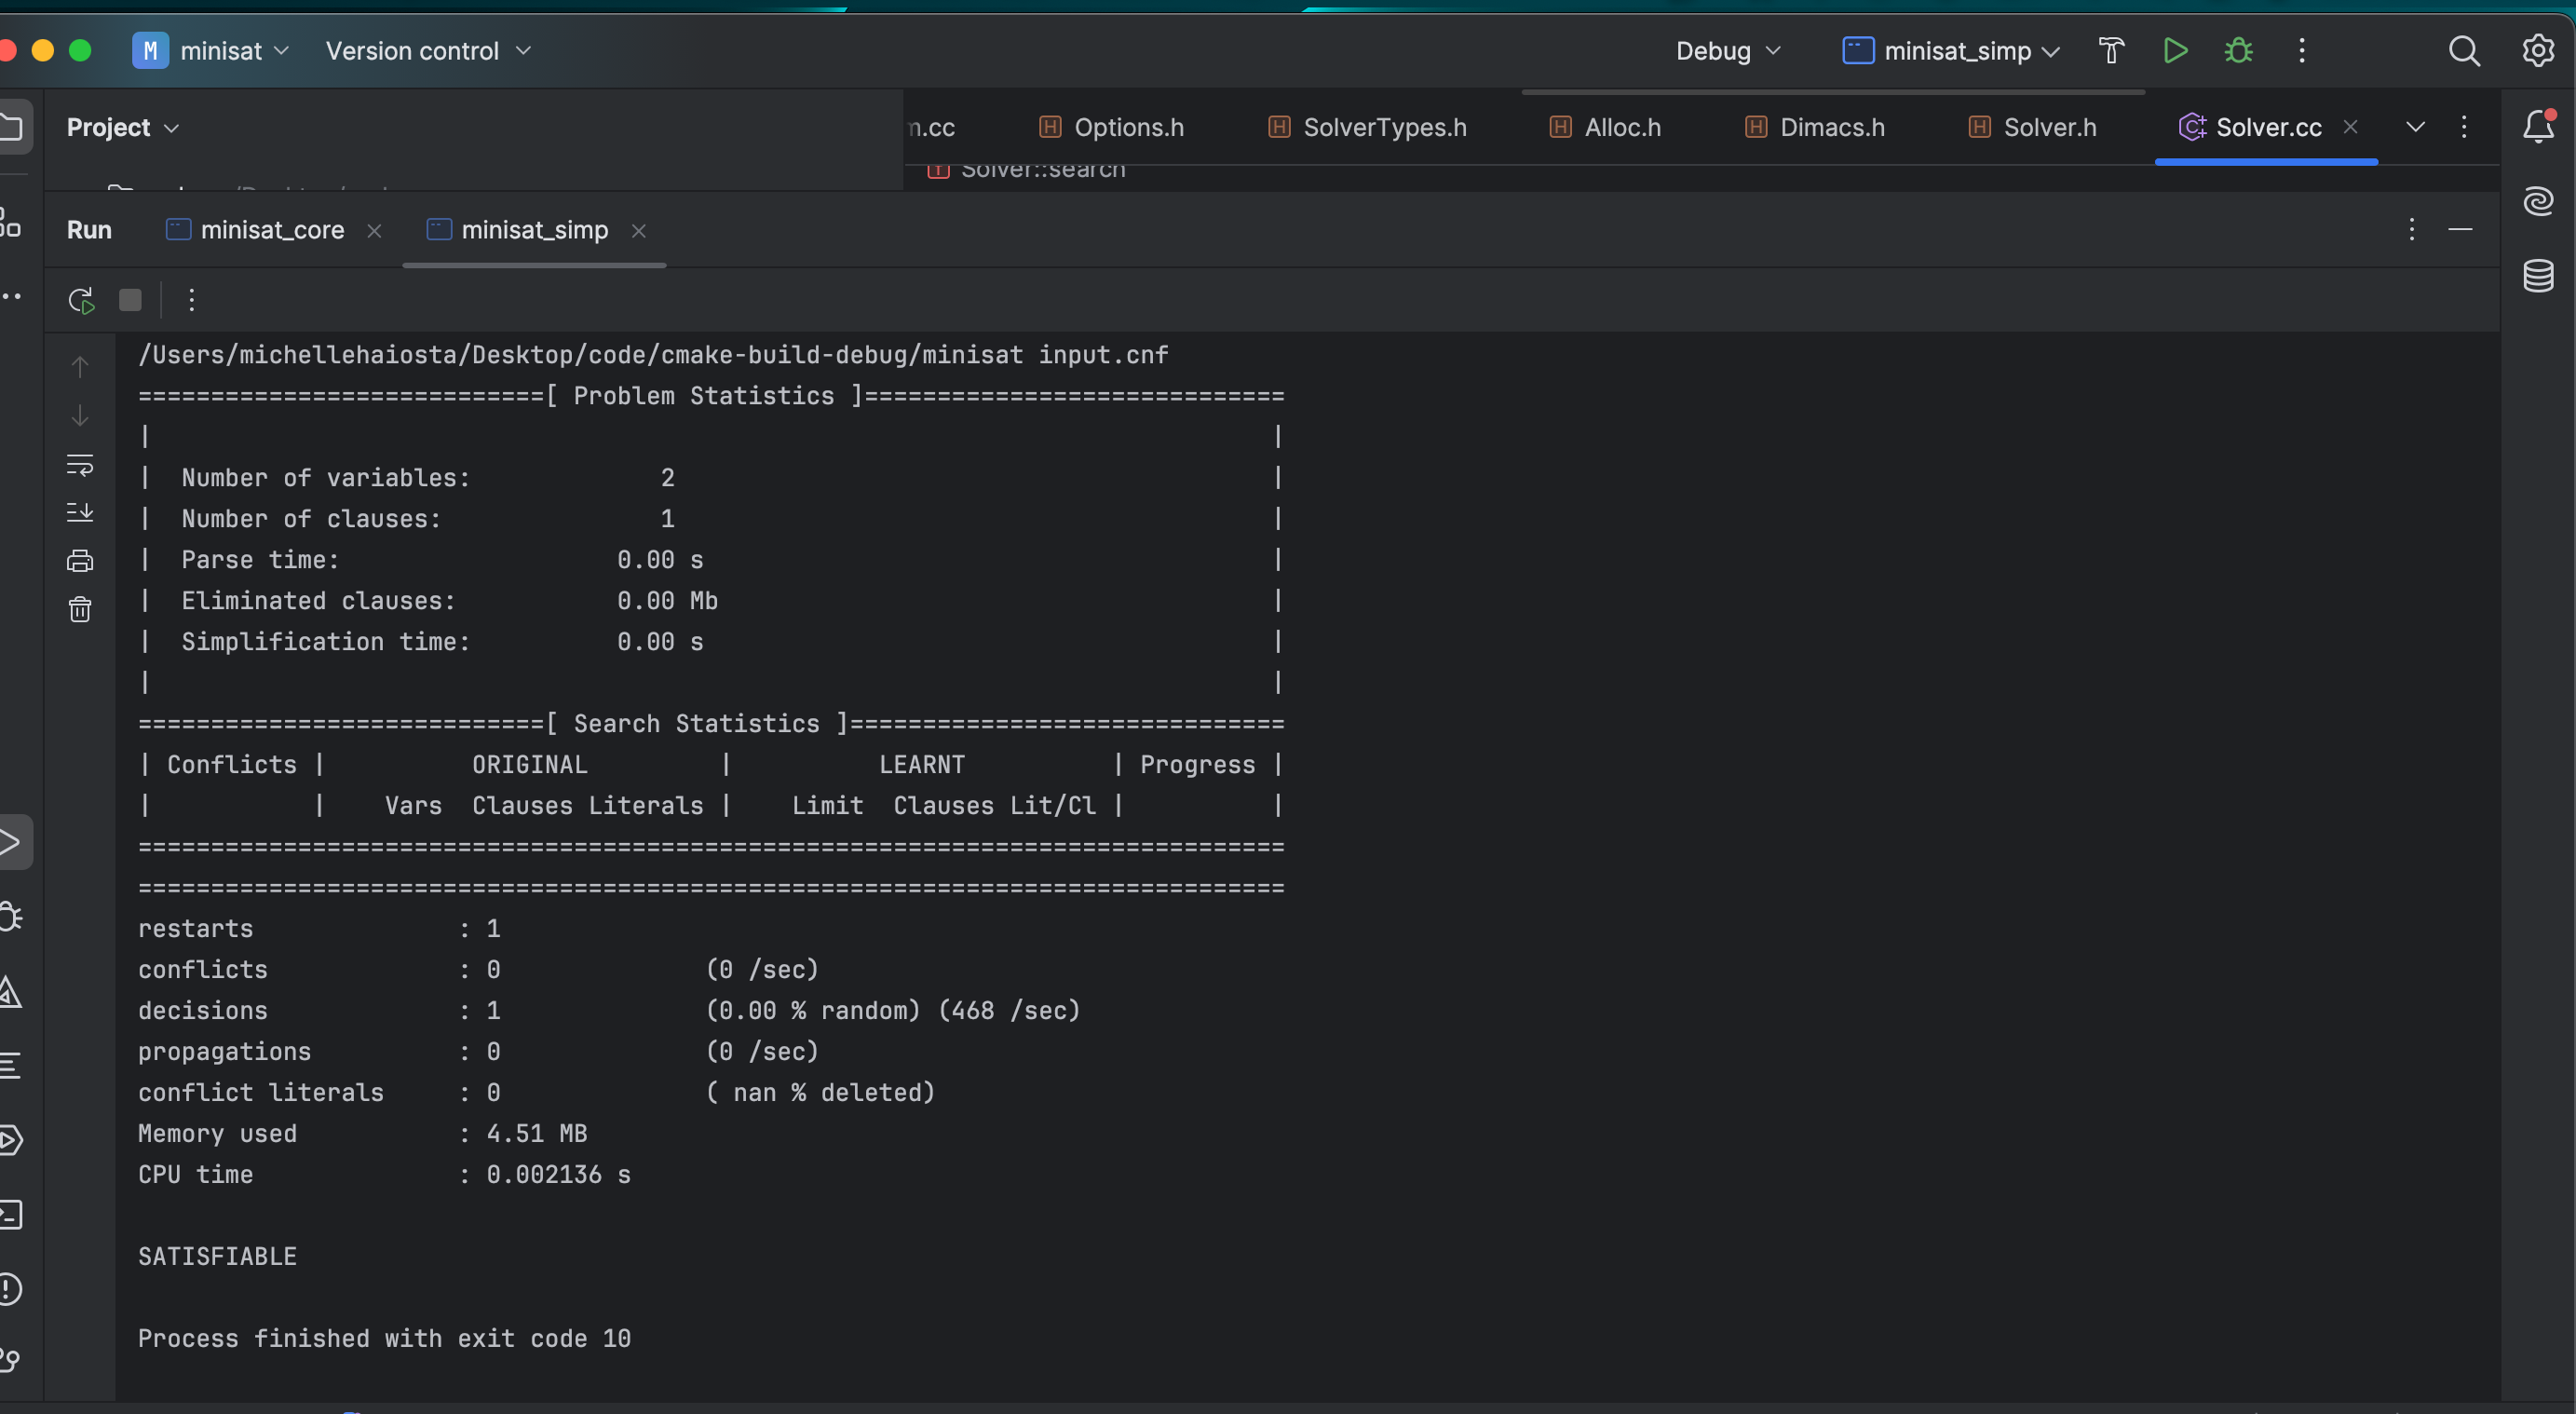
\includegraphics[width=0.75\linewidth]{images/minista.png}
    \caption{Rezultatul execuției generat de MiniSat}
    \label{fig:2}
\end{figure}

MiniSat oferă două categorii principale de informații: statistici despre problemă și detalii privind execuția programului.

Statistici despre problemă: Solverul a identificat două variabile și o singură clauză logică în problema specificată. Fișierul input.cnf a fost citit și procesat aproape instantaneu (Parse time: 0.00 s), fără a elimina clauze redundante sau a necesita timp suplimentar pentru simplificare.

Detalii despre execuție: Solverul a efectuat un singur restart și nu a întâmpinat conflicte, ceea ce indică faptul că problema a fost simplă și bine definită. Cu o singură decizie luată și fără propagări suplimentare, algoritmul a găsit rapid soluția. Consumul de memorie a fost minim (4.51 MB), iar timpul de procesare a fost extrem de scurt (0.001 s).

Rezultatul final: Solverul a determinat că problema este SATISFIABILĂ, ceea ce înseamnă că o configurație validă a variabilelor satisface condițiile specificate în fișierul de input.
\subsection{Analiza etapei de debug – Funcția Solver::search}

În această etapă, am analizat comportamentul funcției Solver::search din cadrul proiectului MiniSat utilizând breakpoint pentru a înțelege fluxul de execuție și starea variabilelor. Această funcție este responsabilă de găsirea unei soluții satisfiabile sau de confirmarea nesatisfiabilității problemei.

Funcția Solver::search se ocupă de procesarea clauzelor, luarea deciziilor și propagarea acestora în cadrul algoritmului SAT. La momentul analizei, am configurat inputul ca fișierul input.cnf, plasând fișierul în directorul cmake-build-debug, și am setat acest director ca Working Directory în configurația de rulare. Fișierul CNF utilizat conținea o problemă simplă pentru a facilita înțelegerea procesului.

\textbf{Breakpoint la linia 788}

\begin{figure}
    \centering
    \includegraphics[width=0.75\linewidth]{images/Captură de ecran din 2025-01-26 la 15.58.15.png}
    \caption{debug Search}
    \label{fig:2}
\end{figure}

La începutul funcției Solver::search, solverul inițializează variabilele necesare procesării problemei.

nof\underline{}conflicts este setată la 100. Aceasta definește limita maximă de conflicte acceptate înainte de a efectua un restart. Este o măsură de control care ajută solverul să gestioneze eficient explorarea.

backtrack\underline{}level are o valoare mare (16082616 în cazul nostru). Acest lucru indică faptul că, la momentul inițial, solverul nu se află într-o stare de conflict și nu are nevoie să revină la niveluri anterioare pentru a reevalua deciziile.
Concluzie: Această etapă confirmă că solverul este pregătit să proceseze problema fără conflicte inițiale, iar toate variabilele relevante sunt corect setate pentru procesarea ulterioară.

\textbf{Breakpoint la linia 837}

\begin{figure}
    \centering
    \includegraphics[width=0.75\linewidth]{images/Captură de ecran din 2025-01-26 la 18.57.03.png}
    \caption{debug Solver}
    \label{fig:2}
\end{figure}

La acest punct, solverul verifică dacă este necesară simplificarea clauzelor. Procesul de simplificare reduce redundanțele și optimizările clauzelor pentru a accelera rezolvarea:

Condiția evaluată este decisionLevel() == 0 and !simplify(). Aceasta verifică dacă solverul se află la nivelul de decizie 0 (fără decizii recente) și dacă există clauze care pot fi simplificate.

În cazul nostru:

Simplificarea nu este necesară, deoarece problema este simplă, iar clauzele sunt deja optimizate.

Solverul continuă procesarea fără a efectua modificări suplimentare.
Variabile observate la acest punct:

learnt\underline{}clause: Aceasta este goală (NULL), ceea ce indică faptul că solverul nu a întâlnit conflicte și, astfel, nu a fost nevoie să învețe sau să deducă clauze noi.

conflict: Valoarea rămâne 0, confirmând că solverul nu a identificat contradicții în procesul de propagare sau decizie.


\section{Propuneri de îmbunătățiri pentru metodele MiniSat}  
MiniSat este un solver puternic pentru problema SAT, dar, ca orice algoritm, poate fi optimizat. În continuare, sunt prezentate câteva direcții posibile de îmbunătățire. \cite{een2006sat} \cite{heule2015efficient}

\subsection{Învățarea clauzelor conflictuale}  
În metoda \textbf{analyze()}, MiniSat învață clauze noi din conflictele pe care le întâlnește, astfel încât să evite conflictele similare în viitor. Acest proces funcționează foarte bine, dar, pe măsură ce solverul rulează, baza de date de clauze devine foarte mare, ceea ce poate încetini algoritmul.

O posibilă îmbunătățire ar fi introducerea unei analize mai detaliate a clauzelor învățate. De exemplu, dacă o clauză nu a fost utilizată într-o propagare recentă, aceasta este probabil inutilă și poate fi eliminată. În plus, putem optimiza clauzele învățate reducând numărul de literali din ele. Clauzele mai compacte sunt mai rapide de utilizat în propagare, dar trebuie să fim atenți să nu pierdem informații importante.

\subsection{Curățarea bazei de date de clauze}  
Metoda \textbf{reduceDB()} elimină periodic clauzele învățate care nu mai sunt utile, dar procesul actual se bazează pe reguli fixe. De exemplu, clauzele cu activitate scăzută sunt șterse automat, indiferent dacă mai sunt relevante sau nu.

Propunem o metodă mai dinamică de curățare a bazei de date. În loc să ștergem toate clauzele sub un anumit prag de activitate, putem evalua cât de des au fost utilizate recent în propagare. Clauzele care nu au fost folosite deloc în ultimele iterații ar putea fi șterse mai întâi. De asemenea, putem curăța doar o parte din baza de date la fiecare iterație, pentru a evita încetinirea solverului.

\subsection{Optimizarea propagării} 
Propagarea unitară este unul dintre cele mai importante procese din algoritmul MiniSat, dar și unul dintre cele mai costisitoare din punct de vedere al timpului de execuție. În timpul propagării, solverul verifică clauzele pentru a vedea dacă setările actuale ale variabilelor determină anumiți literali să fie adevărați sau falși. Pentru a face acest lucru eficient, MiniSat folosește liste „watch” pentru literali, un mecanism care urmărește doar doi literali din fiecare clauză. Totuși, acest proces poate fi optimizat prin îmbunătățirea structurii listei „watch”.

În forma actuală, listele „watch” sunt implementate astfel încât fiecare literal să fie asociat cu un set de clauze în care este urmărit. Acest lucru funcționează bine pentru probleme mai mici, dar pentru formule mari, cu milioane de clauze și variabile, accesarea și actualizarea acestor liste poate deveni lentă. 
De exemplu, de fiecare dată când un literal devine fals, solverul trebuie să parcurgă clauzele asociate acestuia pentru a găsi un alt literal valid care să fie urmărit.

Să considerăm următoarea formulă SAT simplă în forma normală conjunctivă (CNF):
\[
C_1: (x_1 \lor \neg x_2 \lor x_3)
\]
\[
C_2: (\neg x_1 \lor x_4)
\]
\[
C_3: (x_2 \lor \neg x_4 \lor x_5)
\]

În această formulă, fiecare clauză conține literali care pot fi fie o variabilă (\(x_1, x_2, \dots\)) fie negarea unei variabile (\(\neg x_1, \neg x_2, \dots\)). La începutul algoritmului, MiniSat selectează doi literali din fiecare clauză pentru a-i urmări. De exemplu, în \(C_1\), ar putea fi selectați \(x_1\) și \(\neg x_2\) ca literali „watch”. Acest lucru permite solverului să monitorizeze doar o parte din clauză, reducând astfel numărul de verificări necesare pentru propagare.

În timpul execuției, dacă solverul decide că \(x_1 = \texttt{False}\), clauzele care urmăresc \(x_1\) trebuie reevaluate. Pentru \(C_1\), \(x_1\) fiind fals, solverul trebuie să găsească un alt literal valid care să fie urmărit, cum ar fi \(x_3\). Acest lucru asigură că \(C_1\) rămâne satisfăcută. În mod similar, pentru \(C_2\), dacă \(x_1 = \texttt{False}\), \(x_4\) devine singurul literal „watch” valid. Dacă \(x_4\) este ulterior setat la \texttt{False}, clauza \(C_2\) devine conflictuală, iar solverul trebuie să gestioneze acest conflict.

Deși aceste liste „watch” sunt eficiente în reducerea numărului de verificări, accesarea și actualizarea lor poate fi un proces costisitor în cazul problemelor de mari dimensiuni. Fiecare literal are asociată o listă de clauze, iar atunci când un literal devine fals, solverul trebuie să parcurgă toate clauzele asociate pentru a găsi un alt literal valid. Acest proces poate consuma mult timp, mai ales dacă numărul de clauze este mare.

Pentru a aborda această problemă, o posibilă optimizare este utilizarea unei structuri de date mai eficiente, cum ar fi un \textbf{hash map}. În loc ca listele „watch” să fie stocate ca vectori, fiecare literal poate fi o cheie într-un hash map, iar valorile asociate să fie listele de clauze. Această structură permite accesarea și actualizarea mai rapidă a clauzelor asociate unui literal. De exemplu, pentru formula de mai sus, un hash map ar putea fi organizat astfel:

\[
\text{Literal } x_1: \{C_1, C_2\}
\]
\[
\text{Literal } x_2: \{C_1, C_3\}
\]
\[
\text{Literal } x_3: \{C_1\}
\]
\[
\text{Literal } x_4: \{C_2, C_3\}
\]
\[
\text{Literal } x_5: \{C_3\}
\]

Această organizare reduce timpul necesar pentru accesarea clauzelor și face propagarea mai eficientă. Mai mult, pentru formule mari, unde fiecare literal poate fi asociat cu mii de clauze, utilizarea unui hash map asigură o scalabilitate mai bună și minimizează impactul creșterii dimensiunii formulei asupra performanței solverului.
\section{Prezentarea metodelor cheie din MiniSat prin diagrame UML}  

\subsection{propagate()}  
\begin{center}[H]
    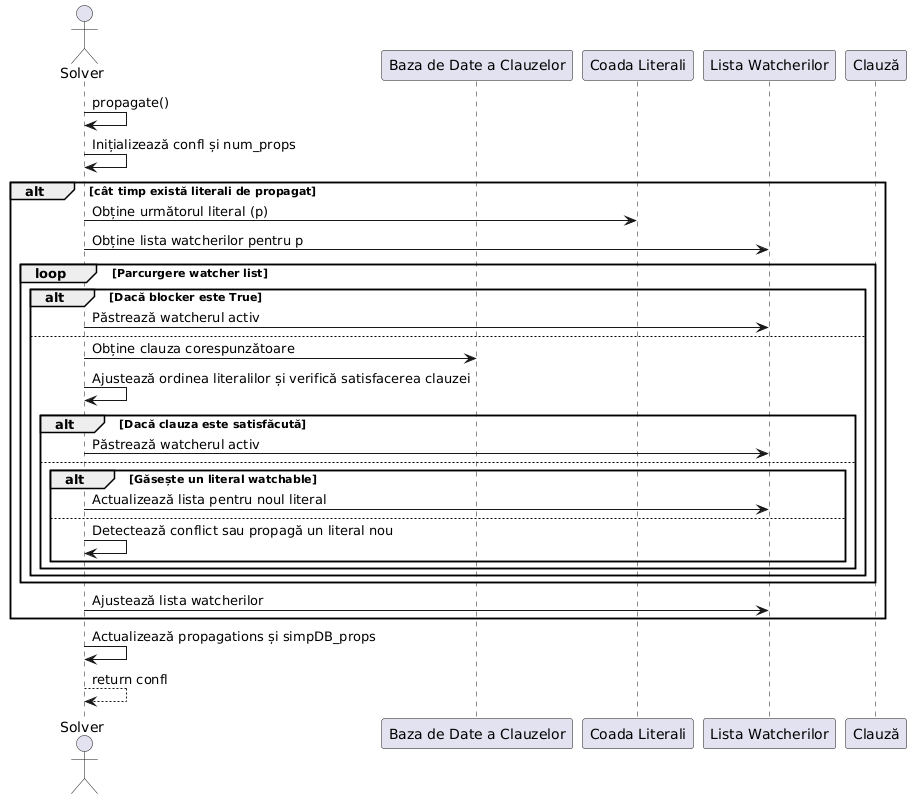
\includegraphics[width=1.0\textwidth]{images/diagrams/pseudo_code/propagate_romana_2.png}
    \caption{Diagrama de secvențe pentru metoda propagate}
    
\end{center}  

Funcția \textbf{propagate()} este una dintre cele mai importante componente ale MiniSat, responsabilă pentru realizarea propagării unitare și pentru identificarea conflictelor. Această funcție parcurge coada de propagare, care conține literalii ce trebuie procesați. Pe baza acestor literali, se examinează clauzele asociate pentru a decide dacă există deducții noi ce pot fi făcute sau dacă a apărut un conflict.

\paragraph{Descriere detaliată a funcției propagate():}  
La început, funcția verifică dacă coada de propagare conține literali neprocesați. Dacă coada este goală, funcția se încheie, indicând că nu mai există deducții de făcut. În caz contrar, se selectează un literal din coadă și se examinează clauzele asociate acestuia.  

Pentru fiecare clauză, funcția verifică dacă starea variabilelor permite deducerea unui nou literal. Dacă o clauză are toți literalii evaluați ca fiind falși, se generează un conflict, iar funcția returnează referința la această clauză. În schimb, dacă un literal al clauzei rămâne nesatisfăcut, acesta este dedus ca fiind adevărat, iar propagarea continuă.  

Acest proces se repetă până când fie coada de propagare devine goală, fie un conflict este detectat. Funcția \textbf{propagate()} joacă un rol crucial în eficiența algoritmului, deoarece permite reducerea spațiului de căutare prin deducții automate și identificarea rapidă a contradicțiilor.

Inițializarea procesului

Când funcția propagate() este apelată, se inițializează variabilele necesare pentru proces. Variabila confl este setată inițial la NULL, ceea ce indică faptul că nu există conflicte la începutul propagării. În același timp, num\underline{ }props este utilizată pentru a contoriza numărul de literali procesați pe parcursul execuției funcției.

Coada de propagare, care conține literalii ce trebuie evaluați, este preluată pentru a începe procesul de propagare. Această coadă reprezintă punctul central al propagării unitare.

Procesarea cozii de propagare
Funcția începe să proceseze coada de propagare iterativ. Pe rând, fiecare literal din coadă este extras și procesat. Pentru fiecare literal, se obține lista de „watchers” (supraveghetori) asociați cu acesta. Watcherii sunt structuri care indică clauzele ce trebuie verificate atunci când un literal este modificat.

Analiza clauzelor asociate
Pentru fiecare literal extras, se parcurge lista clauzelor asociate, verificând starea fiecărei clauze:

Dacă clauza este satisfăcută deja, watcherul asociat este păstrat activ. Acest lucru înseamnă că nu este necesar să se facă modificări în această clauză, deoarece condiția sa este îndeplinită.
Dacă clauza nu este satisfăcută, se verifică ceilalți literali din clauză pentru a găsi un „literal watchable” (un literal care poate deveni adevărat). Dacă un astfel de literal este găsit, lista watcherilor este actualizată pentru a include noul literal și procesul continuă.
Dacă nu există literali watchable în clauză și aceasta devine unitară (toți ceilalți literali sunt falși), funcția propagă literalul unitar, adăugându-l în coada de propagare.
Dacă clauza devine complet falsă (niciun literal nu poate fi satisfăcut), se identifică un conflict. În acest caz, variabila confl este actualizată pentru a semnala conflictul și procesul de propagare se încheie. Actualizarea datelor și ieșirea din funcție.

Pe măsură ce funcția procesează fiecare literal, variabila num\underline{}props este incrementată pentru a reflecta numărul total de literali procesați. După ce coada de propagare este complet procesată, funcția returnează fie NULL (dacă propagarea s-a încheiat fără conflicte), fie o referință la clauza în care a fost detectat conflictul.
\newpage
\subsection{analyse()}
\begin{center}
    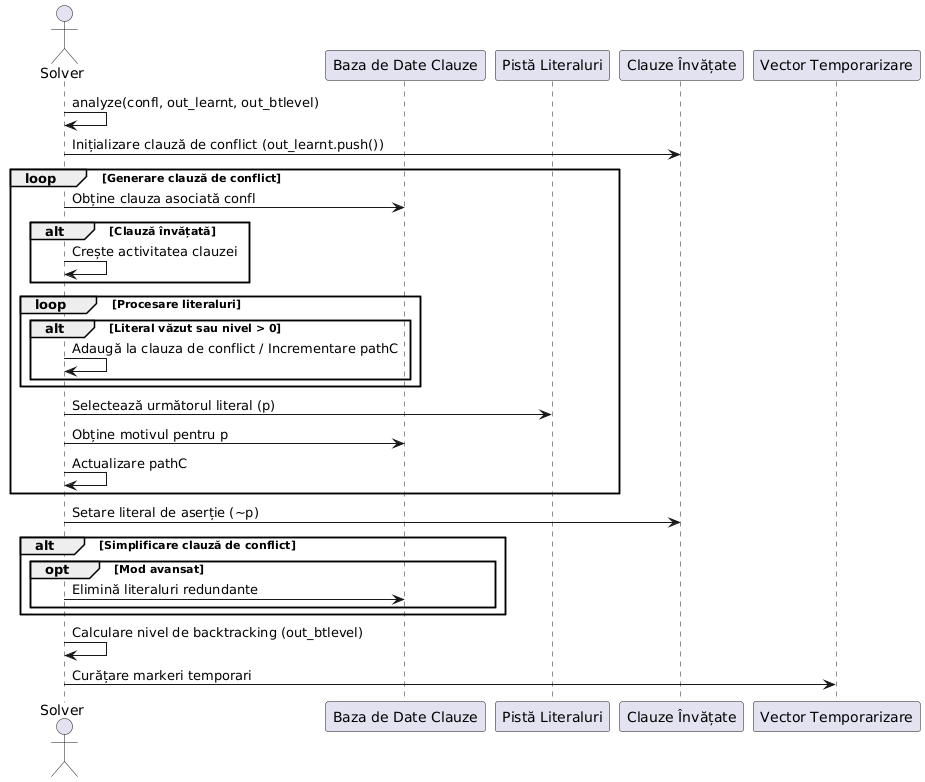
\includegraphics[width=1.0\textwidth]{images/diagrams/pseudo_code/analyze_romana_2.png}
     \caption{Diagrama de secvențe pentru metoda analyze}
\end{center}
Funcția analyse() din MiniSat se ocupă cu înțelegerea motivului pentru care apare un conflict și ajută solver-ul să învețe din greșeli, astfel încât să nu facă aceleași erori în viitor. Când solver-ul întâlnește un conflict, funcția este chemată pentru a analiza situația și pentru a crea o clauză nouă, numită clauza învățată, care va ajuta la evitarea acelui conflict data viitoare. Totul începe prin a verifica variabilele implicate în conflict pentru a înțelege ce decizii au dus la problemă.

Pe baza acestor informații, funcția creează clauza învățată, care conține doar variabilele importante legate de conflict. Această clauză este adăugată în baza de date a solver-ului, astfel încât să împiedice reapariția aceleiași situații. În același timp, funcția decide și până la ce pas anterior trebuie să se întoarcă solver-ul pentru a corecta problema, fără să ia de la capăt tot procesul. În loc să reia totul de la zero, solver-ul se întoarce doar până la pasul necesar pentru a continua corect.

La final, funcția analyse() returnează două lucruri: clauza învățată, care este salvată în baza de date, și pasul la care solver-ul trebuie să revină. Această funcție este importantă pentru că ajută solver-ul să rezolve problemele mai repede și să evite să repete greșelile.

\subsection{reduceDb()}
\begin{center}
    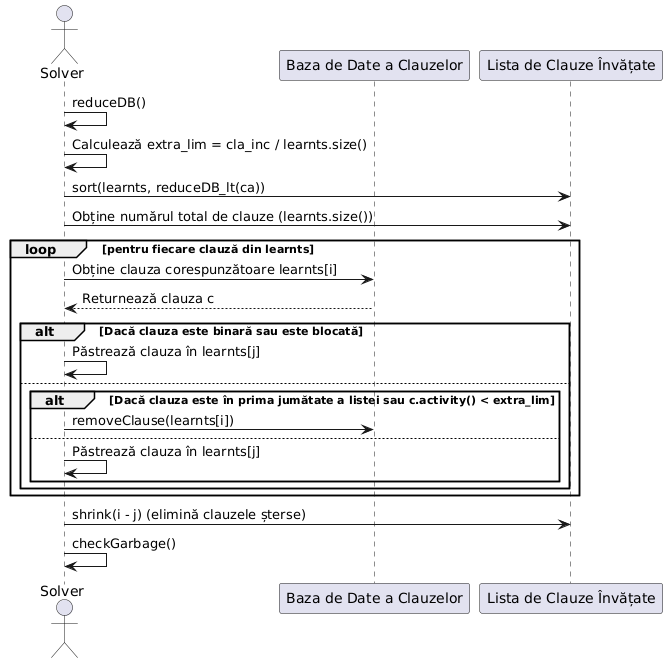
\includegraphics[width=1.0\textwidth]{images/diagrams/pseudo_code/reduceDb_romana.png}
       \caption{Diagrama de secvențe pentru metoda reduceDb}
\end{center}
Funcția reduceDB() are rolul de a menține solverul eficient și rapid prin eliminarea clauzelor învățate care nu mai sunt utile. La început, calculează un prag de activitate (extra\underline{}lim) care ajută la identificarea clauzelor relevante. Apoi, ordonează clauzele învățate astfel încât cele mai puțin importante să fie analizate primele. Clauzele care sunt binare sau blocate sunt păstrate deoarece ajută foarte mult în procesul de deducere. În schimb, clauzele mai puțin active sau cele aflate în prima jumătate a listei sunt eliminate pentru a nu aglomera solverul. La final, funcția actualizează lista de clauze și curăță memoria, astfel încât MiniSat să funcționeze mai eficient și să evite supraîncărcarea cu informații inutile.

\section{Cum colaborează DPLL cu CDCL în implementare}
În implementarea unui solver SAT modern, precum Minisat, metodele tradiționale de rezolvare a problemei satisfiabilității booleene, cum ar fi DPLL (Davis-Putnam-Logemann-Loveland), sunt combinate cu tehnici avansate de învățare a clauzelor bazate pe CDCL (Conflict-Driven Clause Learning). Cele două metode lucrează împreună pentru a accelera căutarea soluției, îmbunătățind eficiența algoritmului și minimizând numărul de conflicte și propagări necesare pentru a rezolva problema SAT \cite{biere2012conflict}

\subsection{DPLL: Algoritmul de bază}

Algoritmul DPLL este un algoritm recursiv care extinde metoda de backtracking pentru a rezolva problemele SAT. DPLL are la bază câteva operații esențiale:

Decizii: Algoritmul face alegeri ale variabilelor, atribuie valori (adevărat sau fals) acestora și se asigură că toate clauzele sunt satisfăcute. Dacă o clauză nu este satisfăcută, se face o decizie de backtrack, încercând o altă valoare pentru variabila respectivă.
Propagare unitară: Când o variabilă este atribuită, aceasta poate determina alte variabile să aibă un anumit sens în contextul clauzelor. Propagarea unitară se referă la procesul de propagare a acestor decizii prin toate clauzele implicate.
Backtracking: Dacă se ajunge la un punct în care nu există niciun mod de a satisface clauzele, algoritmul face backtracking pentru a modifica deciziile anterioare și a încerca soluții alternative.
Totuși, DPLL are limitările sale, în special când vine vorba de gestionarea unui număr mare de clauze și de conflictele care apar. De aici apare necesitatea îmbunătățirii aduse de CDCL.

\subsection{CDCL: Învățarea de clauze și gestionarea conflictelor}

CDCL extinde DPLL prin integrarea tehnicii de învațare a clauzelor conflictuale și utilizarea unui restart dinamic pentru a îmbunătăți performanța căutării soluției.

Principalele elemente ale CDCL includ:

Învățarea clauzelor: Când apare un conflict, CDCL analizează conflictul și învață o nouă clauză care reflectă acea contradicție. Această clauză este adăugată în baza de date a clauzelor și este folosită pentru a preveni conflictele similare în viitor. În esență, CDCL „învăță” din conflictele întâlnite, îmbunătățind căutarea.
Backtracking bazat pe conflict: În loc de a face backtracking simplu (ca în DPLL), CDCL efectuează un backtracking bazat pe conflict. Acest lucru înseamnă că atunci când apare un conflict, solverul caută să identifice care decizii anterioare au contribuit la conflict și revine doar la acele decizii, eliminând astfel opțiunile care nu ar fi putut duce niciodată la o soluție satisfăcătoare.
Restart dinamic: CDCL introduce și restarturi dinamice, care ajută la evitarea impasurilor în care solverul rămâne blocat. Aceste restarturi ajută la eficientizarea căutării prin resetarea anumitor părți ale algoritmului și încercarea unor noi căi de explorare. \cite{audemardsimon2009glucose}
\subsection{Integrarea DPLL cu CDCL}

DPLL formează baza algoritmului SAT, iar CDCL adaugă optimizări semnificative pentru a îmbunătăți performanța generală. Cele două componente sunt interdependente și colaborează în mod continuu pentru a rezolva problema satisfiabilității. Într-o implementare de tip CDCL, cum este Minisat, DPLL este folosit pentru a face decizii și pentru a propaga valorile atribuite variabilelor, dar CDCL adaugă un strat suplimentar de învățare și gestionare a conflictelor.

\subsection{Deciziile și Propagările}
Într-un solver CDCL, procesul începe printr-o decizie de variabilă, realizată folosind aceleași tehnici ca în DPLL. O variabilă este aleasă și i se atribuie o valoare. Acesta este punctul în care DPLL „intervine”, selectând variabilele care urmează a fi atribuite.

După ce decizia este făcută, propagarea este efectuată pentru a determina dacă această decizie determină un conflict sau duce la noi decizii. Dacă nu există conflicte, algoritmul continuă cu noile decizii, în mod similar cu DPLL.

\subsection{Învățarea Clauzelor Conflictuale}
Dacă un conflict apare în timpul propagării, CDCL adaugă o componentă suplimentară: învățarea clauzelor conflictuale. Algoritmul analizează conflictul, identifică sursa acestuia și creează o clauză de conflict care reflectă contradicția întâlnită. Acesta este un proces complex de analyze care îmbunătățește căutarea prin adăugarea unei clauze care va preveni aceleași conflicte în viitor.

Odată ce clauza de conflict este învățată, solverul efectuează un backtracking bazat pe conflict. Spre deosebire de DPLL, care revine la niveluri de decizie arbitrare, CDCL revine la un nivel de decizie mai înalt (nivelul care a contribuit la conflict), eliminând ramuri ale căutării care nu vor duce niciodată la o soluție validă.

\subsection{Restarturi și Performanță}
Într-un solver DPLL, algoritmul ar continua să exploreze aceleași ramuri, indiferent de câte ori întâlnește un blocaj. În schimb, CDCL introduce restarturi dinamice, care resetează anumite părți ale algoritmului pentru a evita blocajele pe termen lung. Aceste restarturi sunt ghidate de o secvență de Luby și sunt utilizate pentru a explora căi alternative într-o manieră mai eficientă. Restarterile sunt aplicate doar atunci când solverul ajunge într-un punct în care nu mai există progres.

\newpage

\subsection{Beneficiile Colaborării DPLL cu CDCL}

Colaborarea dintre DPLL și CDCL aduce mai multe beneficii:

Îmbunătățirea performanței: Prin utilizarea învățării clauzelor, CDCL permite solverului să evite conflictele care ar fi apărut din nou, reducând semnificativ timpul de calcul.
Explorarea mai eficientă a spațiului de soluții: CDCL folosește restarturi dinamice și backtracking bazat pe conflict pentru a evita blocajele și a eficientiza căutarea.
Reducerea dimensiunii bazei de date a clauzelor: În CDCL, clauzele conflictuale care nu sunt folosite de mult timp sunt eliminate, ceea ce reduce memoria utilizată și îmbunătățește performanța.
 
\section{Challenges}
Datorită optimizărilor deja existente, orice îmbunătățire trebuie gândită foarte bine, deoarece modificările care funcționează bine pentru un tip de probleme pot să nu fie la fel de eficiente pentru alte tipuri. De exemplu, dacă introducem o nouă strategie pentru selectarea variabilelor, aceasta poate accelera foarte mult rezolvarea formulelor cu puține clauze, dar același algoritm ar putea să încetinească semnificativ performanța pentru formule mai complexe sau mai mari. Acest tip de compromis face ca procesul de îmbunătățire să fie unul sensibil și care necesită o analiză detaliată. Performanța unui solver SAT nu depinde doar de modul în care sunt implementați algoritmii, ci și de caracteristicile formulelor pe care le rezolvă. De exemplu, o formulă cu foarte multe clauze scurte ar putea beneficia de o tehnică diferită față de o formulă cu mai puține clauze, dar mai lungi. De aceea, pentru a evalua cu adevărat efectul unei modificări, este nevoie de un set extins de teste, care să includă formule din diferite categorii.

Pe partea de benchmark, pot apărea provocări în momentul gestionării unei probleme complexe cu număr mare de variabile și clauze. Se poate ajunge la un spațiu de căutare mare și o rezolvare mai lentă, necesitând mai multe restarturi și decizii. De asemenea, timpul de procesare poate depăși limita alocată, mai ales în cazul problemelor cu dificultate sporită, rezultatul rămânând "indeterminate", ceea ce sugerează că algoritmii de căutare nu sunt suficient de rapizi sau eficienți pentru astfel de situații.

\newpage

\bibliographystyle{ieeetr} % Style for bibliography (e.g., plain, plainnat, IEEEtran)
\bibliography{references} % Name of the .bib file (without .bib extension)

\section{Contributii}
\begin{enumerate}
    \item Haiosta Michelle si Bosna Marinel: Analiza codului, Propuneri de imbunatatiri ale codului in MiniSat, Challenges, Diagrame
    \item Popovici Adrian Robert: Rulare Benchmark
    \item Cerean Bogdan-Ioan: Introducere, Descrierea problemei, Instalare MiniSat
\end{enumerate}

Link-ul spre repository-ul de GitHub: https://github.com/rainman226/minisat



\end{document}